\documentclass[10pt,a4paper]{article}

% ---------- Codificación e idioma ----------
\usepackage[utf8]{inputenc}
\usepackage[T1]{fontenc}            % acentos y guiones bien en el PDF
\usepackage[english]{babel}
\DeclareUnicodeCharacter{2212}{-} % el signo menos Unicode no rompe la compilación

% ---------- Página ----------
\usepackage[a4paper,margin=2cm]{geometry}   % 2 cm: límite de 2 páginas
\usepackage{microtype}              % mejor reparto de espacios, ahorra líneas
\usepackage{multicol}

% ---------- Matemáticas ----------
\usepackage{amsmath,amssymb,amsthm}

% ---------- Unidades y química ----------
\usepackage{siunitx}
\sisetup{per-mode=symbol}           % kcal/mol en vez de kcal mol^-1
\DeclareSIUnit\calorie{cal}         % ¡usar \kilo\calorie, no \kilo\cal!
\DeclareSIUnit\atm{atm}
\DeclareSIUnit\hartree{\ensuremath{E_\mathrm{h}}}
\usepackage[version=4]{mhchem}

% ---------- Figuras y tablas ----------
\usepackage{graphicx}
\usepackage{booktabs}
\usepackage{float}
\usepackage[font=small,labelfont=bf]{caption}
\usepackage{tikz}
\usepackage{pgfplots}
\pgfplotsset{compat=1.18}

% ---------- Otros ----------
\usepackage[normalem]{ulem}         % normalem: \emph sigue siendo cursiva

% ---------- Compactación (para el límite de 2 páginas) ----------
\usepackage{titling}                % título más compacto
\setlength{\droptitle}{-1.6cm}
\pretitle{\begin{center}\large\bfseries}\posttitle{\par\end{center}\vspace{-0.6em}}
\preauthor{\begin{center}\normalsize}\postauthor{\par\end{center}\vspace{-0.9em}}
\predate{\begin{center}\small}\postdate{\par\end{center}\vspace{-1.2em}}
\usepackage{titlesec}               % secciones con menos espacio alrededor
\titleformat{\section}{\large\bfseries}{\thesection}{0.6em}{}
\titlespacing*{\section}{0pt}{1.1ex plus 0.3ex}{0.5ex}
\usepackage[shortlabels]{enumitem}  % listas sin espacios extra
\setlist{nosep, leftmargin=*}
\setlength{\intextsep}{6pt plus 2pt minus 2pt}       % espacio alrededor de figuras/tablas [H]
\captionsetup{skip=4pt}
\setlength{\parskip}{0pt}
\usepackage{etoolbox}               % bibliografía más pequeña y sin huecos
\apptocmd{\thebibliography}{\footnotesize\setlength{\itemsep}{0pt}\setlength{\parsep}{0pt}}{}{}

% ---------- Referencias (siempre al final y en este orden) ----------
\usepackage[hidelinks]{hyperref}
\usepackage[capitalise,noabbrev]{cleveref}



\title{The reaction field, not the dielectric constant:\\solvent effects on the Menshutkin reaction \ce{H3N + CH3Cl}}
\author{Martín Llorens Giménez\thanks{\textbf{Declaration of AI use:} An AI assistant (Claude Opus 5.5, Anthropic) was consulted for editorial assistance to refine English phrasing and grammar, as well as to assist in writing a bash script for log file parsing and generating figure/table plotting code. All calculations, data processing, and intellectual content are the author's sole responsibility.}}
\date{November 2026}


\begin{document}

\maketitle

\section{Introduction}

In a Menshutkin reaction an amine attacks an alkyl halide to give a
quaternary ammonium salt~\cite{Menschutkin1890}. Unlike a conventional
\ce{S_{N}2}, it starts from two neutral molecules and ends in two ions, so
charge is not displaced but \emph{created} along the reaction coordinate.
The Hughes--Ingold rules~\cite{Hughes1935} therefore predict a large
acceleration by polar solvents, and experiment confirms it: the rate spans
more than four orders of magnitude from hydrocarbons to dipolar aprotic
solvents~\cite{Reichardt2011}.

The exercise reported here~\cite{guion7} asks for the activation barrier,
the transition state (TS) geometry and the charge on the leaving chloride
to be correlated with the dielectric constant $\varepsilon$ of the medium.
However, $\varepsilon$ is a macroscopic property of the bulk liquid and
does not appear on its own in any expression for the energy of the solute.
In a continuum model the solvent is a structureless dielectric in which the
solute carves a cavity; the solute polarises the medium, and the polarised
medium acts back on it through a reaction field~\cite{Tomasi2005}. For the
analytically solvable case of a point dipole in a spherical cavity,
Onsager~\cite{Onsager1936} obtained
$\Delta G_\mathrm{solv} = -(\mu^{2}/a^{3})\,f(\varepsilon)$ with
$f(\varepsilon) = (\varepsilon-1)/(2\varepsilon+1)$, so that $\varepsilon$
enters only inside a \emph{bounded} function, $0 \leq f < 1/2$; the Born
and Kirkwood expressions share this feature~\cite{Kirkwood1934}. The
mapping $\varepsilon \rightarrow f(\varepsilon)$ therefore compresses the
polar end of the scale severely: acetonitrile and water differ by 43 units
in $\varepsilon$ but by 0.011 in $f(\varepsilon)$.

The hypothesis of this work is that the apparent saturation of solvent
effects with $\varepsilon$ is an artefact of the chosen variable: plotted
against $f(\varepsilon)$, the same quantities should be linear, and the
resulting straight line should have predictive value for any solvent of
known $\varepsilon$. The Onsager expression is used here to identify the
variable, not to compute anything.



\section{Methods}

All calculations used Gaussian~09~\cite{gaussian09} at the HF/6-31+G*
level, the diffuse functions being required by the chloride anion and by
the charge separation in the transition state (TS). Solvation was described
with the polarizable continuum model~\cite{Tomasi2005}, in which the solute
polarises a structureless dielectric whose induced surface charges act back
on it. SMD~\cite{Marenich2009} was deliberately avoided: it adds terms
parametrised from solvent descriptors other than $\varepsilon$, which would
confound a test of whether a single electrostatic variable governs the
solvent dependence. Heptane, benzene, chloroform, acetonitrile and water
were used, with the gas phase as the $\varepsilon = 1$ limit fixing the
origin of the $f(\varepsilon)$ axis; the dielectric constants are those
applied internally by the program, not the nominal values of the handout.
The reactant complex, the TS, the reactants \ce{NH3} and \ce{CH3Cl} and the
products \ce{CH3NH3+} and \ce{Cl-} were optimized in each medium and
characterised by harmonic frequencies, chained through the six media from
the converged geometry of the previous one; every minimum gave real
frequencies only and every TS exactly one imaginary frequency. Barriers are
referred to the separated reactants, the only reference available in all
six media and the one matching the second-order rate constants measured
experimentally.

Atomic charges are not observables, and any partition of a continuous
density among atoms is a convention. Mulliken populations~\cite{Mulliken1955}
assign each basis function to the atom on which it is centred, which with
diffuse functions no longer reflects where the density is; charges were
therefore obtained with ChelpG~\cite{Breneman1990}, a fit to the molecular
electrostatic potential, the same quantity that generates the reaction
field. Relative rates follow from
$k_\mathrm{rel} = \exp(-\Delta\Delta G^{\ddagger}/RT)$ at
\SI{298.15}{\kelvin}; data were extracted from the output files with an
\texttt{awk} script.

\section{Results and discussion}
\label{sec:results}

\textbf{The effect does not saturate; the axis does.} Correlated against
$\varepsilon$, as the exercise requests, none of the six quantities in
\cref{tab:data} is linear: $R^{2}$ lies between 0.45 and 0.58, and the
barrier shows the familiar saturation above $\varepsilon \approx 30$
(\cref{fig:main}a). Against $f(\varepsilon)$, every one of them becomes a
straight line, $0.977 \leq R^{2} \leq 0.9998$. Same points, same
calculations: only the abscissa changes.

\textbf{A predictive model.} The five solvents define
$\Delta G^{\ddagger} = -32.2\,f(\varepsilon) + 43.6$~kcal/mol
($R^{2} = 0.996$), which gives the barrier of any solvent from its
dielectric constant alone to within 1.5~kcal/mol in a leave-one-out test.
The reactant complex is not an alternative reference: the dipole--dipole
interaction holding it is screened by the medium, and beyond benzene the
surface is flat; where it does exist it lies \emph{above} the separated
reactants in free energy.

\textbf{An earlier, less polarised transition state.} Both $q$(Cl) and
$\mu$ \emph{decrease} with solvent polarity: the TS is less polarised in
water than in vacuum, the opposite of what direct polarisation would give.
The cause is geometric. The reaction yields two separated ions and is
endergonic by \num{114.09}~kcal\,mol$^{-1}$ in the gas phase, but
solvation of those ions makes it exergonic by acetonitrile
(\cref{fig:main}d), a swing of \num{129}~kcal\,mol$^{-1}$. Hammond's
postulate then demands an earlier TS, and $d$(N--C) lengthens from
\num{1.899} to \SI{2.209}{\angstrom} while $d$(C--Cl) shortens from
\num{2.474} to \SI{2.289}{\angstrom} (\cref{fig:main}c); an earlier TS has
transferred less charge. The geometric displacement overrides the direct
polarisation. The Leffler coefficient
$\alpha = \partial\Delta G^{\ddagger}/\partial\Delta G_\mathrm{r} = 0.15$
confirms a reactant-like TS, and the reaction turns exergonic above
$\varepsilon \approx 8$, consistent with these alkylations being run in
acetonitrile or DMSO rather than in hydrocarbons.

\textbf{One variable, five correlations.} These correlations are not
independent. The only solvent property entering a continuum calculation is
$\varepsilon$, and only through $f(\varepsilon)$; if every property of the
solute is linear in that single variable, each is linear in the others. The
Hammond ($R^{2} = 0.996$) and Leffler ($R^{2} = 0.9995$) relations follow
from that common dependence rather than testing it, and only their slopes
carry independent information. The conclusion does not depend on the charge
partition scheme: Mulliken charges differ in absolute value, \num{-0.700}
against \num{-0.790} in the gas phase, but show the same trend and the same
contrast, $R^{2} = 0.62$ against $\varepsilon$ and \num{0.99} against
$f(\varepsilon)$.

\begin{table}[H]
  \centering
  \caption{TS geometry, ChelpG charge on chlorine, dipole moment, barrier
    (from the separated reactants) and reaction free energy. The last two
    rows give $R^{2}$ of a linear fit of each column against $\varepsilon$
    and against $f(\varepsilon)$.}
  \label{tab:data}
  \footnotesize
  \setlength{\tabcolsep}{4pt}
  \begin{tabular}{l S[table-format=2.4] S[table-format=1.3]
                    S[table-format=1.3] S[table-format=1.3]
                    S[table-format=-1.3] S[table-format=2.2]
                    S[table-format=2.2] S[table-format=-3.2]}
    \toprule
    Medium & {$\varepsilon$} & {$f(\varepsilon)$} & {$d$(N--C)} &
    {$d$(C--Cl)} & {$q$(Cl)} & {$\mu$} &
    {$\Delta G^{\ddagger}$} & {$\Delta G_\mathrm{r}$} \\
     & & & {\si{\angstrom}} & {\si{\angstrom}} & {$e$} & {D} &
    \multicolumn{2}{c}{kcal\,mol$^{-1}$} \\
    \midrule
    Gas          &  1.0000 & 0.000 & 1.899 & 2.474 & -0.790 & 13.51 & 47.67 &  114.09 \\
    Heptane      &  1.9113 & 0.189 & 2.035 & 2.396 & -0.774 & 12.89 & 37.78 &   51.43 \\
    Benzene      &  2.2706 & 0.229 & 2.061 & 2.381 & -0.771 & 12.77 & 36.11 &   40.59 \\
    Chloroform   &  4.7113 & 0.356 & 2.136 & 2.335 & -0.761 & 12.37 & 31.68 &   10.85 \\
    Acetonitrile & 35.6880 & 0.479 & 2.203 & 2.292 & -0.749 & 12.00 & 28.24 &  -12.97 \\
    Water        & 78.3553 & 0.490 & 2.209 & 2.289 & -0.748 & 11.96 & 27.97 &  -14.93 \\
    \midrule
    $R^{2}$ vs.\ $\varepsilon$    & {--} & {--} & 0.510 & 0.527 & 0.576 & 0.549 & 0.447 & 0.464 \\
    $R^{2}$ vs.\ $f(\varepsilon)$ & {--} & {--} & 0.995 & 0.998 & 0.999 & 1.000 & 0.977 & 0.983 \\
    \bottomrule
  \end{tabular}
\end{table}

\begin{figure}[H]
  \centering
  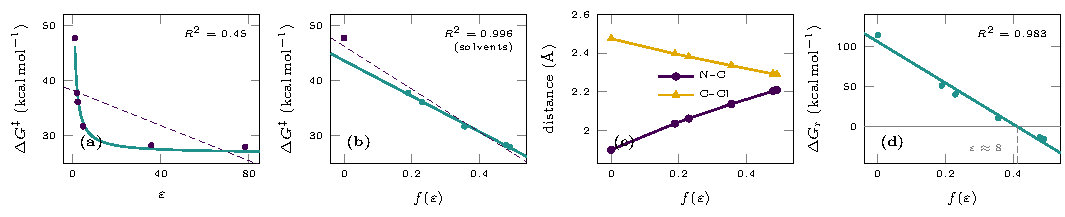
\includegraphics[width=0.98\textwidth]{figura_s7.pdf}
  \caption{(a) Barrier against $\varepsilon$: a linear fit fails
    ($R^{2} = 0.45$); the solid line is the model of (b) mapped onto this
    axis. (b) The same barriers against $f(\varepsilon)$; dashed, the fit
    including the gas phase. (c) TS bond distances and (d) reaction free
    energy against $f(\varepsilon)$.}
  \label{fig:main}
\end{figure}

\section{Conclusion}

Correlating against $\varepsilon$, as requested, gives no linear
relationship for any of the six quantities studied
($0.45 \leq R^{2} \leq 0.58$); against $f(\varepsilon)$ all of them are
linear ($R^{2} \geq 0.977$). The apparent saturation of solvent effects is
a property of the axis, not of the chemistry, and the resulting line
predicts the barrier of any solvent from $\varepsilon$ alone to within
1.5~kcal/mol. Since $f(\varepsilon)$ is the only solvent variable a
continuum model contains, the correlations requested are in fact one
correlation, and only their slopes inform. Those slopes are chemically
sensible: the solvent swings the reaction free energy by 129~kcal/mol,
turning it exergonic above $\varepsilon \approx 8$, and displaces the TS
earlier, leaving it \emph{less} polarised in water than in vacuum. The
model reproduces the direction and order of magnitude of the experimental
effect (9.5 against 5.6~kcal/mol) but overestimates it, as expected from a
method without electron correlation and a continuum without hydrogen bonds.


{\footnotesize
\begin{multicols}{2}
\bibliographystyle{unsrt}
\bibliography{bibliografia}
\end{multicols}
}

\end{document}
